\chapter{Praktični rad}

U iBeacon poglavlju spomenuto je kako se tehnologija iBeacon može iskoristiti u gotovo svim situacijama gdje se sadržaj mijenja ovisno o kontekstu prostora, npr. trgovinama, muzejima, bolnicama i sličnim objektima. 
\\
U nastavku poglavlja opisano je kako se tehnologija iBeacon može integrirati u trgovine. 
\\

Za integraciju je potrebno imati postavljene iBeacon uređaje u prostoru, mobilni uređaj sa podrškom za BLE i instaliranom aplikacijom koja može prepoznati BLE, odnosno iBeacon, odašiljače te poslužiteljsku aplikaciju s koje će mobilni uređaj dohvaćati relevantne podatke.  

\section{Poslužiteljska aplikacija - Spree Commerce}

Spree Commerce (u daljnjem tekstu Spree) je elektronička trgovina \engl{e-commerce} otvorenog koda napisana u Ruby on Rails radnom okruženju. 
Rad na Spreeu je počeo 2007. godine, a danas je jedna od najpopularnijih platformi za elektroničku trgovinu. 
Trenutno više od 45 tisuća trgovina koristi Spree. %TODO reff http://spreecommerce.com/storefront 
\\
Odlike Spree rješenja su ogroman broj već implementiranih funkcija koje imaju sve moderne elektroničke trgovine, modularan programski kôd, lakoća dodavanja novih funkcionalnosti te izmjena i konfiguracija postojećih te brojne druge. 
Uz to, za gotovo svaki aspekt sustava dostupan je skup aplikacijsko programskih sučelja što pojednostavljuje integraciju sustava sa drugim tehnologijama (poput integracije sa mobilnim platformama).
\\
U 2013. godini objavljen je Spree Hub čija je funkcija rješavanje dodatnih poslova vezanih za elektroničku trgovinu. 
Neke odlike Spree Huba uključuju rješavanje logističkih problema (prijenos informacija o narudžbi iz trgovine u skladište), olakšana integracija sustava za računovodstvo, olakšana integraciju sustava za korisničku službu i brojne druge.
\\
Spree Hub se može integrirati skupa sa postojećim elektroničkim trgovinama i pri tome je bitno napomenuti da one ne moraju biti temeljene na Spree Commerce rješenju, već mogu biti temeljene na bilo kojoj drugoj platformi elektroničke trgovine (npr. Magento, Shopify i slične). 

\begin{figure}[H]
    \centering
    
\includegraphics[scale=0.60]{pictures/spree_lavazza}
    \caption{Lavazza Store - jedna od mnogobrojnih elektroničkih trgovina koje koriste Spree}
    \label{pic:spreeLavazza}
\end{figure}

Spree je podijeljen na nekoliko ključnih komponenti (tj. Ruby gemova):
\begin{description}[style=nextline]
    \item[spree\_api] Skup aplikacijsko programskih sučelja koji zadovoljavaju REST\footnote{\textit{Representational State Transfer}} principe.
    \item[spree\_frontend] Komponente korisničkog sučelja.
    \item[spree\_backend] Komponente korisničkog sučelja administratora aplikacije.
    \item[spree\_cmd] Komponente sučelja naredbenog retka \engl{command-line interface, CLI}.
    \item[spree\_core] Ključne komponente, sadrži veliku većinu poslovne logike.
    \item[spree\_sample] Primjeri podataka.
\end{description}

Ako programer želi dodati neku od Spree komponenti u svoju postojeću aplikaciju, sve što treba napraviti je dodati željene komponente u Gemfile\footnote{datoteka koja sadrži popis svih Ruby gemova koji se koriste u projektu} te pokrenuti instalaciju.
\\
Najkraći način za instalaciju Spree gema, stvaranje novoga Ruby on Rails projekta i dodavanja Spreea u novostvoreni projekt prikazan je u nastavku (pretpostavlja se da su Ruby i Ruby on Rails prethodno instalirani i ispravno konfigurirani).

% caption=Instalacija Spree projekta, captionpos=t]
\begin{lstlisting}[language=bash, frame=leftline, backgroundcolor=\color{backcolour}, basicstyle=\footnotesize]
$ gem install spree
$ rails _4.0.5_ new moj_projekt
$ spree install moj_projekt
\end{lstlisting}

Spree projekt se pokreće tako da se pozicioniramo u direktorij projekta i tamo pokrenemo server:
\begin{lstlisting}[language=bash, frame=leftline, backgroundcolor=\color{backcolour}, basicstyle=\footnotesize]
$ cd moj_projekt
$ rails server
\end{lstlisting}

\begin{figure}[H]
    \centering
    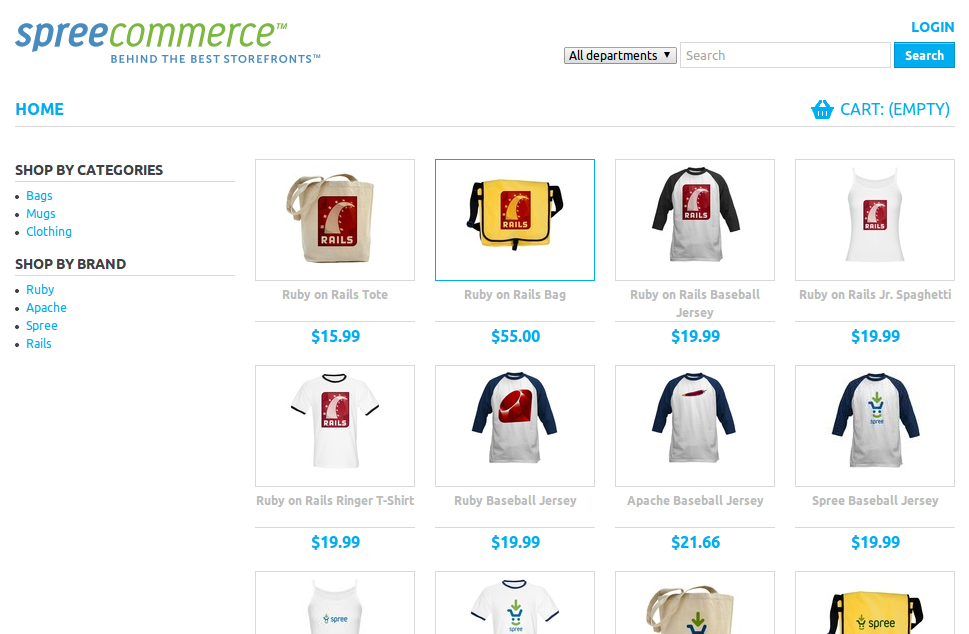
\includegraphics[scale=0.40]{pictures/spree}
    \caption{Početni ekran Spree korisničkog sučelja}
    \label{pic:spree}
\end{figure}

\begin{figure}[H]
    \centering
    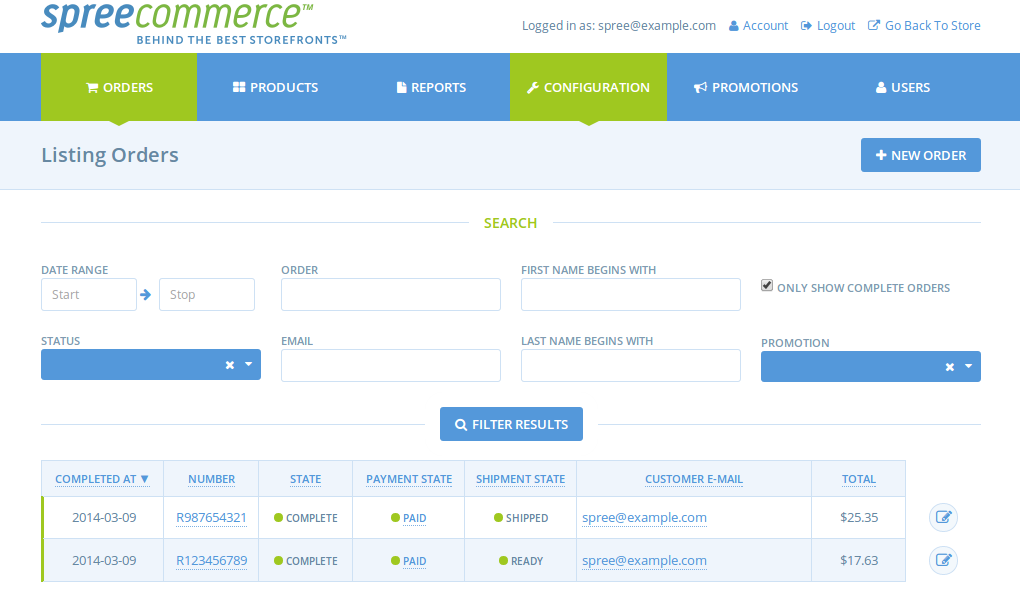
\includegraphics[scale=0.40]{pictures/spree_admin}
    \caption{Početni ekran Spree administratorskog sučelja}
    \label{pic:spree}
\end{figure}

%TODO dijelovi spreea
%Glavna komponenta bilo kojega sustava elektroničke trgovine, a tako i Spreea, je proizvod.
%\\
%U Spreeu svaki proizvod može imati varijante koje se međusobno razlikuju po jednom ili više svojstava (npr. veličini ili boji). 
%Također 

\subsection{Prilagođavanje i nadogradnja}

Modularna arhitektura Spree platforme omogućava jednostavno izmjenu, uklanjanje ili dodavanje novih funkcija u sustav, a kako bi korisničko sučelje bilo optimalno prikazano krajnjim korisnicima Spree nudi i osjetljivi dizajn. 
Postojeći dizajn je također modularan i željeno korisničko sučelje se može jednostavno ostvariti.
\\
Razvijatelji Spree sustava ne preporučuju prethodno spomenuti način prilagođavanja Spreea svojim potrebama, odnosno ne preporuča se izravna izmjena postojećeg programskog kôda Spreea.
Preporučeni način prilagođavanja i nadogradnje Spree sustava je korištenjem takozvanih Spree ekstenzija.

Spree ekstenzija nije ništa drugo nego zasebni Ruby gem kojega se dodaje u Gemfile postojećeg projekta. 
Primjer stvaranja i instaliranja Spree ekstenzije naveden je u nastavku. 
\\

Stvaranje Spree ekstenzije:
\begin{lstlisting}[language=bash, frame=leftline, backgroundcolor=\color{backcolour}, basicstyle=\footnotesize]
$ spree extension moja_ekstenzija
\end{lstlisting}

Za dodavanje ekstenzije u postojeći Spree projekt potrebno je dodati ime i putanju ekstenzije u Gemfile projekta:
\begin{lstlisting}[language=ruby, frame=leftline, backgroundcolor=\color{backcolour}, basicstyle=\footnotesize]
gem 'moja_ekstenzija', path: '../moja_ekstenzija'
\end{lstlisting}

I nakon toga instalirati ekstenziju:
\begin{lstlisting}[language=bash, frame=leftline, backgroundcolor=\color{backcolour}, basicstyle=\footnotesize]
$ bundle install
$ bundle exec rails g moja_ekstenzija:install
\end{lstlisting}

Nadogradnja modela i kontrolera je krajnje jednostavna i ne zahtjeva ponovno pisanje postojećih metoda pojedinih razreda, već se pišu samo nove metode ili metode čiji se sadržaj mijenja. 
\\
Za nadogradnju postojećih pogleda Spree razvojni tim je razvio Deface. 
Deface je biblioteka za jednostavno nadograđivanje, izmjenu i uklanjanje komponenti iz postojećih predložaka. 
Instaliranjem Spree gema, automatski se instalira i Deface. 
Korištenjem Deface biblioteke programer ne mora kompletno mijenjati sve predloške koje njegova ekstenzija nadograđuje, već na elegantan način može dohvaćati pojedine komponente predloška i mijenjati njihov sadržaj.
\\

Prednost ektenzija nad izravnom izmjenom izvornog kôda Spreea je ta što se ostvaruje bolja modularnost kôda, olakšano je ponovno korištenje ekstenzija u drugim projektima te održavanje i nadogradnja sustava sa novim verzijama Spreea je puno jednostavnije. 
Uz to, Spree tim održava i službeni repozitorij\footnote{\url{http://spreecommerce.com/extensions}} gdje se može pronaći veliki broj besplatnih ekstenzija.
\\

Za integraciju iBeacon funkcionalnosti u Spree projekt razvijena je \textit{Spree Taxon Webservice} ekstenzija koja svakoj kategoriji proizvoda dodaje \textit{reference id} atribut. 
Na taj način će se ovisno o vrijednostima identifikatora obližnjeg iBeacon odašiljača prikazivati određena kategorija proizvoda.
\\

Sada mobilni uređaj nakon identifikacije obližnjeg odašiljača može poslati poslužitelju HTTP zahtjev sa pripadnim sadržajem:
\begin{lstlisting}[frame=leftline, backgroundcolor=\color{backcolour}, basicstyle=\footnotesize]
GET /api/products?q[taxons_ref_id_eq]=beaconId
\end{lstlisting}

U slučaju da je detektirano više odašiljača sadržaj zahtjva je:
\begin{lstlisting}[frame=leftline, backgroundcolor=\color{backcolour}, basicstyle=\footnotesize]
GET /api/products?q[taxons_ref_id_in][]=beaconId1
	&q[taxons_ref_id_in][]=beaconId2
\end{lstlisting}

Poslužitelj će kao odgovor poslati JSON objekt sa proizvodima koje pripadni odašiljač (ili odašiljači) referenciraju.

%TODO slika sučelja za dodjelu/izmjenu ref_id

\subsection{Instalacija i pokretanje poslužiteljske aplikacije}

Prije instaliranja i podešavanja poslužiteljske aplikacije potrebno je imati ispravno instaliran i konfiguriran Ruby te instalirane Ruby on Rails, Spree i Bundler Ruby gemove. 
Nakon toga se može stvoriti novi Ruby on Rails projekt i u njega ugraditi funkcionalnost Spree sustava:
\begin{lstlisting}[language=bash, frame=leftline, backgroundcolor=\color{backcolour}, basicstyle=\footnotesize]
$ rails new spree_server_app
$ spree install spree_server_app
$ cd spree_server_app
\end{lstlisting}

Nakon toga je potrebno dodati Spree Taxon Webservice ekstenziju u Gemfile projekta:
\begin{lstlisting}[language=ruby, frame=leftline, backgroundcolor=\color{backcolour}, basicstyle=\footnotesize]
gem 'spree_taxon_webservice', path: '../spree_taxon_webservice'
\end{lstlisting}

I instalirati dotičnu ekstenziju:
\begin{lstlisting}[language=bash, frame=leftline, backgroundcolor=\color{backcolour}, basicstyle=\footnotesize]
$ bundle install
$ bundle exec rails g spree_taxon_webservice:install
\end{lstlisting}

Nakon toga, potrebno je dodati CORS\footnote{\textit{Cross-origin resource sharing}} mehanizam u aplikaciju, kako bi se sadržaj poslužiteljske aplikacije mogao slati vanjskim aplikacijama (tj. aplikacijama iz druge domene). 
Najlakši način za rješavanje dotičnog problema je instalacija \textit{Rack CORS Middleware}\footnote{\url{https://github.com/cyu/rack-cors}} gema:
\begin{lstlisting}[language=bash, frame=leftline, backgroundcolor=\color{backcolour}, basicstyle=\footnotesize]
$ gem install rack-cors
\end{lstlisting}

Dodavanje dotičnog gema u Gemfile projekta:
\begin{lstlisting}[language=ruby, frame=leftline, backgroundcolor=\color{backcolour}, basicstyle=\footnotesize]
gem 'rack-cors', :require => 'rack/cors'
\end{lstlisting}

I konačno, omogućiti \textit{cross-origin} zahtjeve u projektu dodavanjem sljedećeg odsječka u \texttt{Application} razred koji se nalazi u \texttt{app/config/application.rb} datoteci:
\begin{lstlisting}[language=ruby, frame=leftline, backgroundcolor=\color{backcolour}, basicstyle=\footnotesize]
config.middleware.use Rack::Cors do
  allow do
    origins '*'
    resource '*', headers: :any, methods: [:get, :post, :options]
  end
end
\end{lstlisting}

Ukoliko su svi prethodni koraci uspješno izvedeni, aplikacija se može pokrenuti sa sljedećom naredbom:
\begin{lstlisting}[language=bash, frame=leftline, backgroundcolor=\color{backcolour}, basicstyle=\footnotesize]
$ rails server
\end{lstlisting}


\section{Klijentska aplikacija}

%TODO uvod
%TODO integriranje aplikacije sa ibeaconima, use caseovi
%TODO spajanje aplikacije sa serverom
%TODO instalacija i pokretanje aplikacije
%TODO eksperimentalna aplikacija